\documentclass[11pt]{article}
\usepackage{setspace}
\setstretch{1}
\usepackage{amsmath,amssymb, amsthm}
\usepackage{graphicx}
\usepackage{bm}
\usepackage[hang, flushmargin]{footmisc}
\usepackage[colorlinks=true]{hyperref}
\usepackage[nameinlink]{cleveref}
\usepackage{footnotebackref}
\usepackage{url}
\usepackage{listings}
\usepackage[most]{tcolorbox}
\usepackage{inconsolata}
\usepackage[papersize={8.5in,11in}, margin=1in]{geometry}
\usepackage{float}
\usepackage{caption}
\usepackage{esint}
\usepackage{url}
\usepackage{enumitem}
\usepackage{subfig}
\usepackage{wasysym}
\newcommand{\ilc}{\texttt}
\newcommand{\p}{\partial}
\usepackage{etoolbox}
\usepackage{algorithm}
\usepackage{changepage}
% \usepackage{algorithmic}
\usepackage[noend]{algpseudocode}
\usepackage{tikz}


\usetikzlibrary{matrix,positioning,arrows.meta,arrows}
\patchcmd{\thebibliography}{\section*{\refname}}{}{}{}
% \PassOptionsToPackage{hyphens}{url}\usepackage{hyperref}

\providecommand{\myceil}[1]{\left \lceil #1 \right \rceil }
\providecommand{\myfloor}[1]{\left \lfloor #1 \right \rfloor }
\providecommand{\qbm}[1]{\begin{bmatrix} #1 \end{bmatrix}}
\providecommand{\qpm}[1]{\begin{pmatrix} #1 \end{pmatrix}}
\providecommand{\norm}[1]{\left\lVert #1 \right\rVert}
\providecommand{\len}[1]{\left| #1 \right|}
\newcommand{\cmark}{\ding{51}}%
\newcommand{\xmark}{\ding{55}}%

\definecolor{dkgreen}{rgb}{0,0.6,0}
\definecolor{gray}{rgb}{0.5,0.5,0.5}
\definecolor{mauve}{rgb}{0.58,0,0.82}

\lstset{frame=tb,
  language=Python,
  aboveskip=3mm,
  belowskip=3mm,
  showstringspaces=false,
  columns=flexible,
  basicstyle={\small\ttfamily},
  numbers=none,
  numberstyle=\tiny\color{gray},
  keywordstyle=\color{blue},
  commentstyle=\color{dkgreen},
  stringstyle=\color{mauve},
  breaklines=true,
  breakatwhitespace=true,
  tabsize=3
}

\begin{document}


\title{\textbf{CSDS 491: Assignment 4}}

\author{Shaochen (Henry) ZHONG, \ilc{sxz517@case.edu}}

\date{Due and submitted on 04/21/2021 \\ Spring 2021, Dr. Lewicki}
\maketitle

\section*{E1. Multivariate Gaussians}
\section*{E2. Linear Gaussian Models}

\subsection*{2.1.}
% https://math.stackexchange.com/questions/60911/multivariate-normal-difference-distribution
% https://stats.stackexchange.com/questions/9879/addition-of-multivariate-gaussians

Known the characteristic functions of $x$ and $z$ is:

\begin{align*}
    \phi_x(u) &= \exp(i u^T \mu_x - \frac{1}{2} u^T \Sigma_x u) \\
    \phi_z(u) &= \exp(i u^T \mu_z - \frac{1}{2} u^T \Sigma_z u)
\end{align*}

Since $x$ and $z$ are independent, their sum will still conform to the normal distribution. We may confirm it by analysing the characteristic functions of $x + z$, which is $\phi_{x + z}(u) = E(e^{it(x + z)}) = E(e^{itx}) \cdot E(e^{itz}) = \phi_{x}(u) \phi_{z}(u)$, then we have:

\begin{align*}
    \phi_{x + z}(u) &= \phi_{x}(u) \phi_{z}(u) = \exp(i u^T \mu_x - \frac{1}{2} u^T \Sigma_x u) \cdot \exp(i u^T \mu_z - \frac{1}{2} u^T \Sigma_z u) \\
    &= \exp(i u^T (\mu_x + \mu_z) - \frac{1}{2} u^T (\Sigma_x + \Sigma_z) u) \\
    \Longrightarrow \phi_y(u) &= \exp(i u^T \mu_y - \frac{1}{2} u^T \Sigma_y u)
\end{align*}

Thus, we have $p(y) = \mathcal N(\mu_x+\mu_z,\Sigma_x+\Sigma_z)$.


\subsection*{2.2.}

% https://stats.stackexchange.com/questions/30588/deriving-the-conditional-distributions-of-a-multivariate-normal-distribution
% http://www.math.chalmers.se/~rootzen/highdimensional/SSP4SE-appA.pdf
% http://users.stat.umn.edu/~helwig/notes/norm-Notes.pdf
% https://www.coursera.org/lecture/linear-models-2/normal-conditional-distributions-LiHmE

For clarity, we let $p(x, y) = \mathcal N(\mu, \Sigma)$, where:

\begin{align*}
    \mu &= \qbm{\mu_x \\ \mu_y} \\
    \Sigma &= \qbm{\Sigma_{xx} & \Sigma_{xy} \\ \Sigma_{yx} & \Sigma_{yy}}
\end{align*}

Note each of $\Sigma{ab}$ is a matrix of $a \times b$.

We further know that there must be $p(y \mid x) = \mathcal N(\overline{\mu}, \overline{\mu})$, where:

\begin{align*}
    \overline{\mu} &= \mu_y + \Sigma_{yx} \Sigma_{xx}^{-1} (x - \mu_x) \\
    \overline{\Sigma} &= \Sigma_{yy} - \Sigma_{yx} \Sigma_{xx}^{-1}\sigma{yx}
\end{align*}

I don't know if we are expected to show the proof, but here's a trick that can do it rather quickly. Assume $z = y + Ax$ (not to be confused with the $z$ in \textbf{Question 2.1}) with $A = -\Sigma_{yx} \Sigma_{xx}^{-1}$, we have:

\begin{align*}
    cov(z, x) &= cov(y + Ax, x) = cov(y, x) + A \cov(x, x) \\
    &= \Sigma_{yx} + (-\Sigma_{yx} \Sigma_{xx}^-1) \Sigma_{xx} \\
    &\text{Now to deduce $E(y \mid x)$} \\
    \Rightarrow &\begin{cases}
        E(z | x) &= E(z) = E(y + Ax) = \mu_y + A \mu_x = \mu_y -\Sigma_{yx} \Sigma_{xx}^{-1} \mu_x \\
        E(z | x) &= E(y + Ax \mid x) = E(y \mid x) + A E(x \mid x)
    \end{cases} \\
    \Longrightarrow E(y \mid x) &= E(z | x) - A E(x \mid x) = \mu_y -\Sigma_{yx} \Sigma_{xx}^{-1} \mu_x - (-\Sigma_{yx} \Sigma_{xx}^{-1}) x \\
    &= \mu_y + \Sigma_{yx} \Sigma_{xx}^{-1} (x - \mu_x) = \overline{\mu}
\end{align*}


Similarily, we may find out $\overline{\Sigma}$ as (note that $cov(x, y) = cov(y, x)$ for scalar):


\begin{align*}
    var(y \mid x) &= var(z) = var(y + Ax) \\
    &= var(y) + A var(x) A' + A cov(y, x) + cov(x, y) A' \\
    &= \Sigma_{yy} + \Sigma_{yx} \Sigma_{xx}^{-1} \Sigma_{xx} \Sigma_{xx}^{-1} \Sigma_{xy} - \Sigma_{yx} \Sigma_{xx}^{-1} \Sigma_{yx} - \Sigma_{yx} \Sigma_{xx}^{-1} \Sigma_{xy} \\
    &= \Sigma_{yy} + \Sigma_{yx} \Sigma_{xx}^{-1} \Sigma_{xy} - 2 \Sigma_{yx} \Sigma_{xx}^{-1} \Sigma_{xy} \\
    \Longrightarrow \overline{\Sigma}&= \Sigma_{yy} - \Sigma_{yx} \Sigma_{xx}^{-1} \Sigma_{xy}
\end{align*}


As know from \textbf{Exercise 2.1} that $p(y) = \mathcal N(\mu_x+\mu_z,\Sigma_x+\Sigma_z)$ and $p(x) = \mathcal N(\mu_x, \Sigma_x)$, we have $p(y \mid x) = \mathcal N(\overline{\mu}, \overline{\mu})$, where:

\begin{align*}
    \overline{\mu} &= \mu_y + \Sigma_{yx} \Sigma_{xx}^{-1} (x - \mu_x) = \mu_x \mu_z + \Sigma_{yx} \Sigma_{xx}^{-1} (x - \mu_x) \\
    \overline{\Sigma} &=  \Sigma_{yy} - \Sigma_{yx} \Sigma_{xx}^{-1} \Sigma_{xy} = \Sigma_{x} + \Sigma_{z} -\Sigma_{yx} \Sigma_{xx}^{-1} \Sigma_{xy}
\end{align*}

\subsection*{2.3.}

According to \textbf{Exercise 2.1}, for $y = x + z$, we have $y \sim \mathcal N(\mu_x+\mu_z,\Sigma_x+\Sigma_z)$. For the ease of demo, let $\sigma_x = 3$ and $\sigma_z = 4$ so that we may have the nice $\sigma_x^2 + \sigma_z^2 = \sigma_y^2 \Longleftrightarrow 3^2 + 4^2 = 5^2$ relationship. In such case, we may have:




\begin{align*}
    p(x) &= \mathcal N(\mu_x = 0, \Sigma_x = 3^2) \\
    p(y) &= \mathcal N(\mu_y = 1, \Sigma_y = 4^2) \\
    p(z) &= \mathcal N(\mu_x+\mu_z,\Sigma_x+\Sigma_z) = \mathcal N(\mu_x = 1, \Sigma_x = 5^2)
\end{align*}

The plots will look like:


\begin{figure}[H]
    \centering
    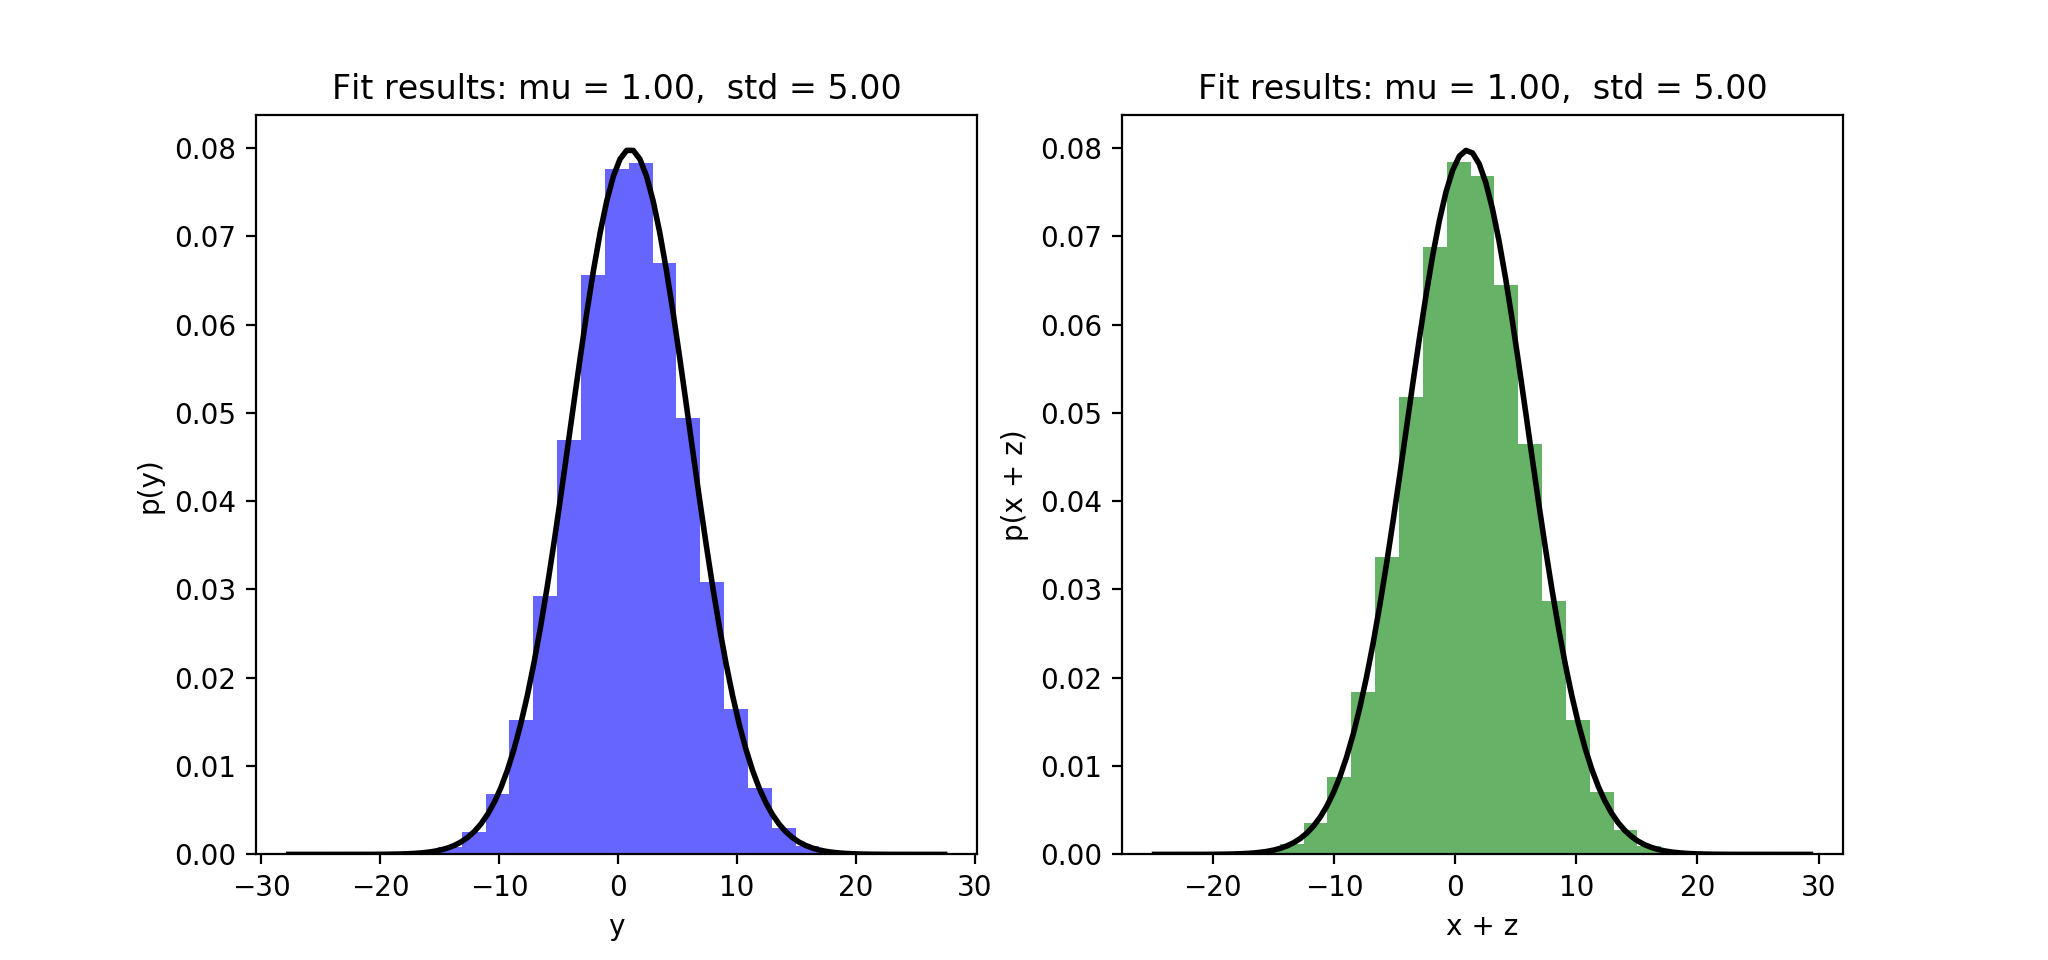
\includegraphics[width=1\linewidth]{{fig/e2.3}.png}
\end{figure}

We may tell these two plots are close resemblance of one and another by inspecting the shape of graph and the parameter of the fitted curve (showed as title of each plot).\newline

Please refer to \ilc{code/p2.py} for the code implementation.

\section*{E3. Dimensionality Reduction and PCA}


\section*{E4. Gaussian Mixture Models }

\end{document}

